\chapter{System Design}

\section{System Architecture}

Halite is a client--server web application (Figure~\ref{fig:architecture}). A React single-page application, hosted on Vercel, calls a FastAPI backend over JSON. The backend runs in Docker on a shared virtual machine and reads and writes a Neo4j graph database. A language model on the Groq API is called by the backend for two jobs only: phrasing an explanation, and proposing a classification for a pair of records. The model never determines the diagnostic ranking.

\begin{figure}[!htbp]
\centering
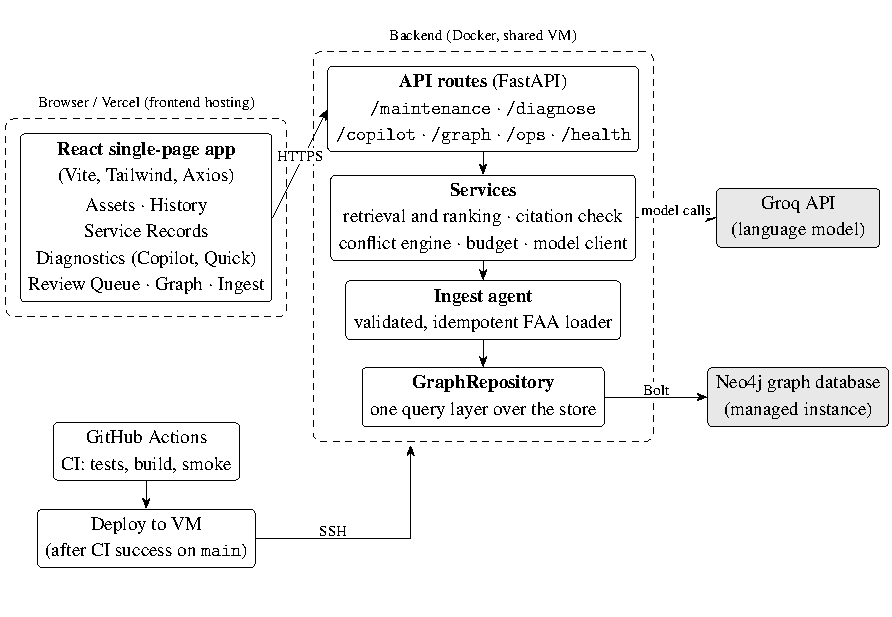
\includegraphics[width=\linewidth,height=0.70\textheight,keepaspectratio]{illustrations/fig_p55_428.pdf}
\caption{System architecture and deployment path. Grey boxes are external services.}
\label{fig:architecture}
\end{figure}

\textbf{Runtime honesty.} \texttt{GET /api/health} reports the graph mode (neo4j or memory), whether the model is live, and the number of records loaded. The application and our evidence documents claim ``real data'' or ``live model'' only when this endpoint agrees. A memory mode exists for tests and degraded operation and is labelled as such.

\textbf{Domain registry.} Domain-specific rules (record labels, source authority) sit behind an adapter. The maintenance adapter is the product; the earlier software-engineering adapter is retained as frozen infrastructure, covered by seven regression tests, and is unreachable from the interface.

\section{Architectural Components}

Table~\ref{tab:components} lists the principal components, their responsibilities and the primary source files.

\begin{table}[H]
\centering
\caption{Components and responsibilities}
\label{tab:components}
\small
\begin{tabularx}{\textwidth}{@{}>{\raggedright\arraybackslash}p{0.22\textwidth} L >{\raggedright\arraybackslash}p{0.28\textwidth}@{}}
\toprule
Component & Responsibility & Main files \\
\midrule
React application & Pages for assets, history, service records, diagnostics, review, graph, ingest; every failure state shown honestly & \texttt{frontend/src/pages}, \texttt{components}, \texttt{utils} \\
API client & One Axios instance and the functions for every endpoint & \texttt{frontend/src/api/client.js} \\
API routes & HTTP contracts, validation, controlled errors (404, 409, 422, 503) & \texttt{backend/api/routes} \\
Ingest agent & Validated, idempotent loading of FAA records; explicit skip counts & \texttt{agents/maintenance\_agent.py} \\
Retrieval and ranking & Bounded graph context; deterministic ranking; copilot context and ranking delta & \texttt{services/diagnostic\_retrieval.py} \\
Citation validation & Extract FAA-shaped identifiers and check them against the graph & \texttt{services/citation\_validation.py} \\
Conflict engine & Candidate pairing, classification, adjudication, confidence, routing & \texttt{services/conflict\_engine.py}, \texttt{conflict\_screen.py} \\
Analysis state and budget & Honest unanalysed state; per-day request and token budget & \texttt{analysis\_state.py}, \texttt{analysis\_budget.py} \\
Model client & Calls Groq; rejects empty content; bounded retries & \texttt{services/groq\_service.py} \\
Graph repository & One query layer over Neo4j or the in-memory store & \texttt{graph/queries.py}, \texttt{schema.py} \\
\bottomrule
\end{tabularx}
\end{table}


\section{Interfaces and Dependencies}

\subsection{Backend interfaces}

Table~\ref{tab:endpoints} summarises the principal backend endpoints and their contracts.

\begin{table}[H]
\centering
\caption{Principal backend endpoints}
\label{tab:endpoints}
\small
\begin{tabularx}{\textwidth}{@{}l >{\ttfamily\raggedright\arraybackslash}p{0.42\textwidth} L@{}}
\toprule
Method & \normalfont Path & Purpose and contract notes \\
\midrule
GET & /api/health & Runtime modes: graph, model, record count \\
GET & /api/maintenance/assets & Fleet list with record counts \\
GET & /api/maintenance/assets/\{id\}/history & Chronological history for one aircraft \\
GET & /api/maintenance/records & Paginated fleet records with filters \\
POST & /api/maintenance/diagnose & One-shot diagnosis; 404 empty history; 503 if model unavailable \\
POST & /api/maintenance/copilot/turn & Multi-turn copilot; client carries case state \\
GET & /api/graph/overview & Nodes and edges for graph view (default node cap 200) \\
GET & /api/maintenance/review-queue & Records awaiting human review \\
POST & /api/maintenance/review-queue/approve & Accept review decision \\
POST & /api/maintenance/review-queue/reject & Reject; note required; 409 if not reviewable \\
GET & /api/maintenance/corrections & Detected SUPERSEDES corrections \\
POST & /api/maintenance/ingest/upload & CSV ingest with confirmation counts \\
POST & /api/maintenance/analysis/run & Bounded batch analysis (ops token) \\
GET & /api/ops/version & Deployed commit identifier \\
GET & /api/ops/logs & Recent log lines (ops token required) \\
\bottomrule
\end{tabularx}
\end{table}

\subsection{Component dependencies}

Figure~\ref{fig:deps} shows which module calls which. Routes call services; services call one repository; the repository is the only code that talks to the database. This keeps the graph queries in one place and lets the same service code run against an in-memory store in tests.

\begin{figure}[!htbp]
\centering
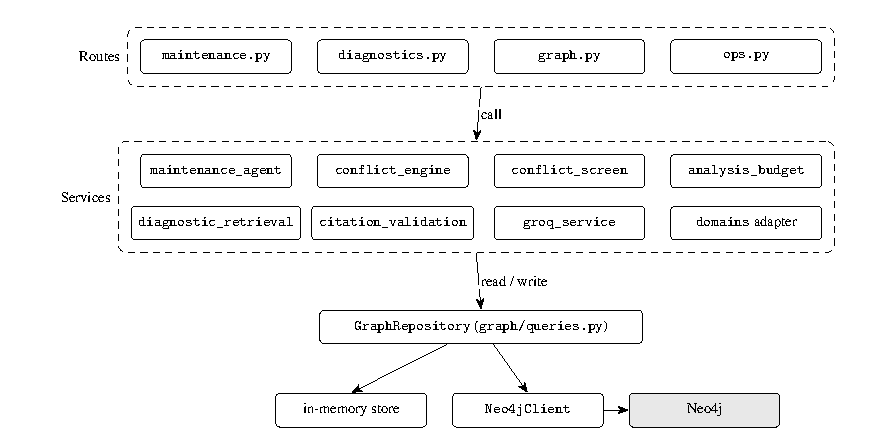
\includegraphics[width=\linewidth,height=0.70\textheight,keepaspectratio]{illustrations/fig_p58_382.pdf}
\caption{Backend component dependencies.}
\label{fig:deps}
\end{figure}

\subsection{External dependencies}

Neo4j (graph database), Groq (language model), FastAPI and Pydantic, pandas (CSV loading), React~18, Vite, Tailwind CSS, Axios, react-force-graph-3d, Vitest, PyTest, Docker Compose, GitHub Actions and Vercel. Section~6.8 gives the list with versions and purpose.

\section{Architecture Decisions and Rationale}

Non-obvious decisions are recorded as short decision records in the repository. Table~\ref{tab:decisions} lists those most relevant to this iteration.

\begin{table}[H]
\centering
\caption{Selected architecture and process decisions}
\label{tab:decisions}
\small
\begin{tabularx}{\textwidth}{@{}>{\raggedright\arraybackslash}p{0.30\textwidth} L@{}}
\toprule
Decision (date) & Rationale \\
\midrule
Maintenance-only frontend (16 Oct) & The product is maintenance diagnostics; legacy software screens stay in the repository but are unreachable \\
Frontend reflects backend outputs (16 Oct) & The interface may add labels and warnings but must never hide, alter or invent a backend value \\
Review actions are server-confirmed (16 Oct) & Accept/reject change real data; the screen updates only after the server confirms \\
Centralised staging and CI-gated release (16 Oct) & One shared staging API; only a commit that passed full CI on main is deployed, with recorded rollback \\
Honest analysis state (17 Oct) & Analysis state is stored separately from confidence; ``unscored'' is never shown as a confident result \\
Fleet-wide paginated records (17 Oct) & Replaced a 119-request fan-out with one paginated, filterable endpoint \\
Opt-in cost cascade (17 Oct) & Pre-registered, off by default: deterministic text screen before the model, then adaptive voting \\
Diagnostic copilot scope waiver (16 Oct) & Limited ownership exception so the copilot could be built across route, retrieval and UI \\
Graph shows one aircraft (17 Oct) & Whole graph is too dense; one aircraft's stored subgraph is readable and every drawn edge is stored \\
Knowledge bank and agent protocol (16 Oct) & Versioned memory of context, flows and decisions updated in the same change as the code \\
\bottomrule
\end{tabularx}
\end{table}


\section{Design Evolution}

Table~\ref{tab:design-evolution} compares the proposal design with what was built at Mid and why.

\begin{table}[H]
\centering
\caption{Design as proposed against design as built}
\label{tab:design-evolution}
\small
\begin{tabularx}{\textwidth}{@{}>{\raggedright\arraybackslash}p{0.18\textwidth} L L@{}}
\toprule
Aspect & Proposal & Built at Mid, and why \\
\midrule
Retrieval & Graph-constrained plus embedding-based hybrid & Graph-bounded with lexical (Jaccard) similarity; embeddings deferred so the baseline is measured first \\
Ranking & Hybrid evidence score with a historical correction penalty & Deterministic: recency and similarity weights, factor 0.3 for superseded records \\
Conflict engine & Five-label classifier with human review & As proposed; plus stored analysis state, daily budget, and opt-in cost cascade after measuring 9{,}175 projected requests \\
Tenancy and identity & PostgreSQL, organisations, roles & Not built; reviewer identity is therefore not recorded \\
Sessions & Server-side diagnostic session storage & Client-side state only; the server is stateless \\
Interface & Chat-centred workspace & Asset-first workspace with a Copilot tab; one-shot diagnose kept as the stable contract \\
Corpus & About 60 airframes & 118 aircraft, because every aircraft with a ground-truth pair is kept first \\
\bottomrule
\end{tabularx}
\end{table}


\section{Domain Model}

Figure~\ref{fig:schema} is the graph schema. There are two node types and three relationship types. Each relationship records its provenance: ABOUT and PRECEDED\_BY are created at ingest; SUPERSEDES is created only by the conflict engine when a supersession is confirmed. No relationship is invented to make the graph look richer; a causal ``component causes failure'' edge is deliberately absent because the data does not justify one.

\begin{figure}[!htbp]
\centering
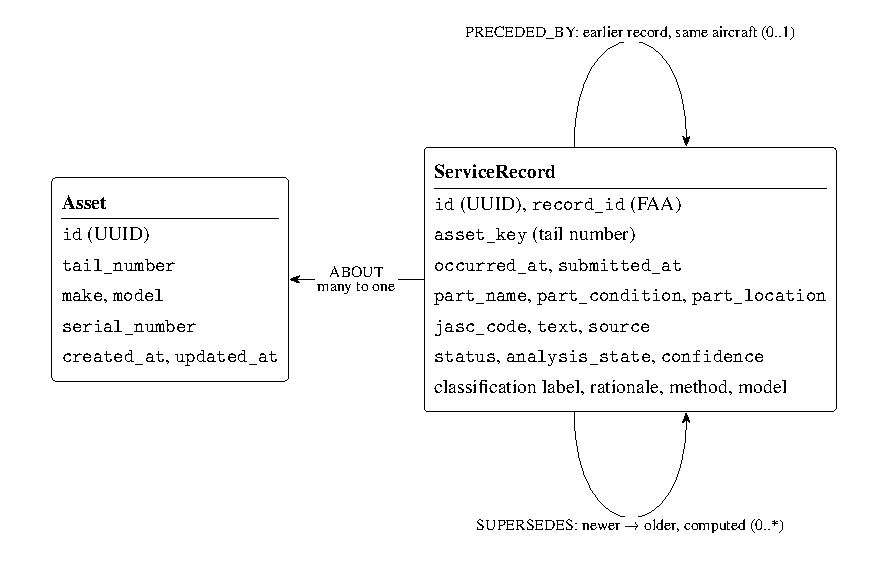
\includegraphics[width=\linewidth,height=0.70\textheight,keepaspectratio]{illustrations/fig_p61_68.pdf}
\caption{Graph schema (entity--relationship view).}
\label{fig:schema}
\end{figure}

\section{Data Design}

\textbf{Source.} FAA Service Difficulty Reports, 2025 file: 67{,}637 raw rows, 66{,}658 after removing duplicates on (aircraft, date, normalised text). The proof-of-concept corpus is a deterministic selection (fixed seed): every aircraft that has a ground-truth pair is included first, then others are added until about 2{,}000 records. It holds 2{,}079 records on 118 aircraft; the largest aircraft has 153 records. Raw and processed files are not committed; a script downloads them \citep{faa2025}.

\textbf{Ground truth.} 141 valid correction pairs written by the FAA reporters (``supplemental report for \ldots'') were extracted; six candidates were discarded (five cite a record outside the corpus, one crosses aircraft).

\textbf{Ingest rules.} A row needs a tail number, a parseable MM/DD/YYYY date and an OperatorControlNumber; otherwise it is counted in a named skip category. A record that already exists is counted as a duplicate and left unchanged, and its ABOUT link is re-asserted so an interrupted earlier run is repaired. New records are stored with status unscored, analysis\_state unscored and a null confidence.

\textbf{Status values.} Workflow status: unscored, no\_action, auto\_accepted, needs\_review, accepted, rejected, superseded. Coverage analysis\_state: unscored, scored, needs\_review, reviewed. The two are separate on purpose: whether a record has been analysed is not the same as what the analysis decided.

\textbf{Known data fact.} On staging, 2{,}079 record nodes have 2{,}078 ABOUT links: one record (AALA202506230216, aircraft 991AU) is an orphan. Re-running ingest repairs it, but staging was not mutated without approval.

\section{Process / Behavior Design}

\subsection{Diagnosis}

Figure~\ref{fig:seq-diagnose} shows the one-shot diagnosis. The retrieval and ranking happen before the model is called, so the ranking is identical with or without a model. If the model is unavailable, or returns empty text, the route returns HTTP~503 with a reason and the interface shows no diagnosis. After the model answers, every identifier in its text is looked up in the graph.

\begin{figure}[!htbp]
\centering
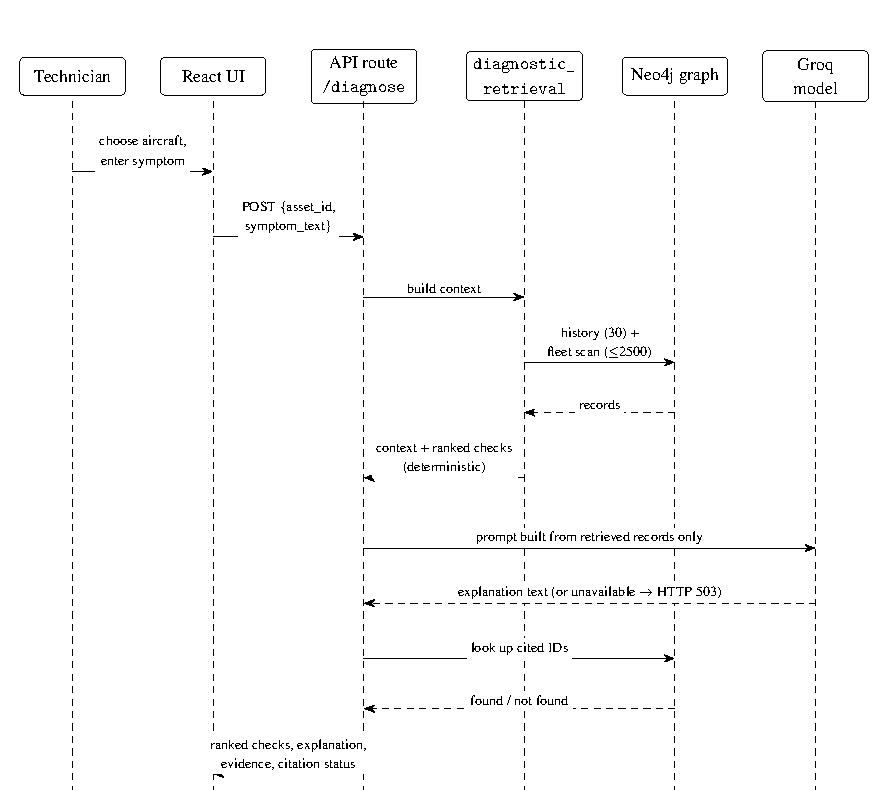
\includegraphics[width=\linewidth,height=0.70\textheight,keepaspectratio]{illustrations/fig_p62_338.pdf}
\caption{Sequence diagram: one-shot diagnosis. Dashed arrows are returns.}
\label{fig:seq-diagnose}
\end{figure}

\subsection{Conflict analysis}

Figure~\ref{fig:activity-conflict} is the conflict pipeline. Only the leftmost path calls the model. Records with no comparable earlier record, and (in cascade mode) pairs the deterministic screen rules out, never reach it.

\begin{figure}[!htbp]
\centering
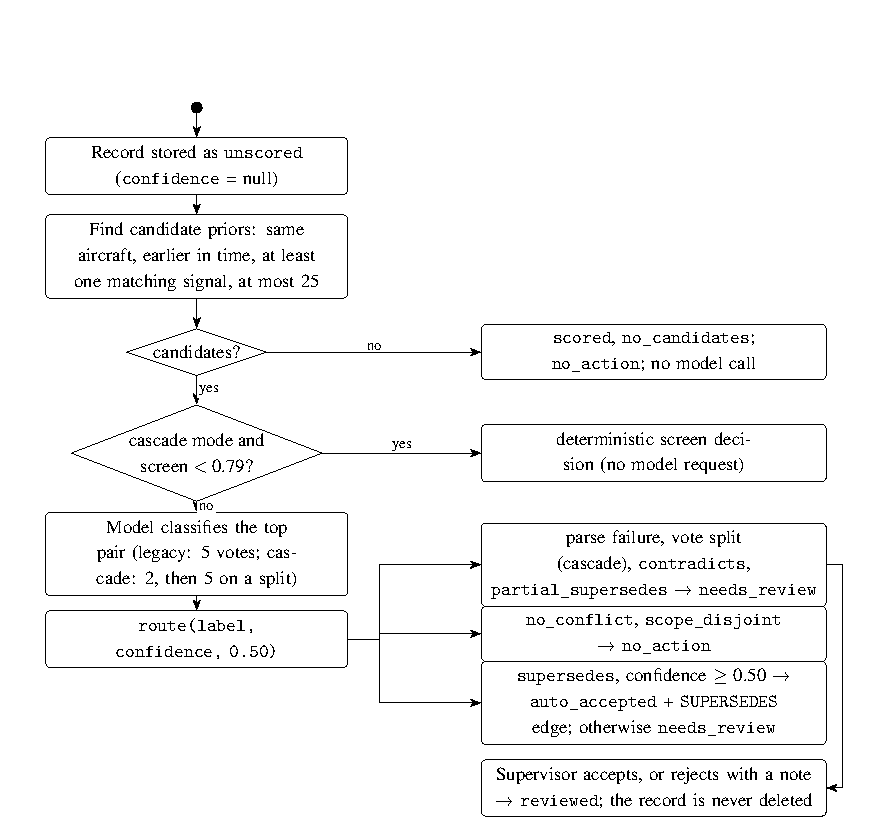
\includegraphics[width=\linewidth,height=0.70\textheight,keepaspectratio]{illustrations/fig_p63_168.pdf}
\caption{Activity diagram: analysis of one record.}
\label{fig:activity-conflict}
\end{figure}

\subsection{Record state}

Figure~\ref{fig:state} shows how the two state fields change. A record's status becomes superseded only when a later record's supersession is confirmed.

\begin{figure}[!htbp]
\centering
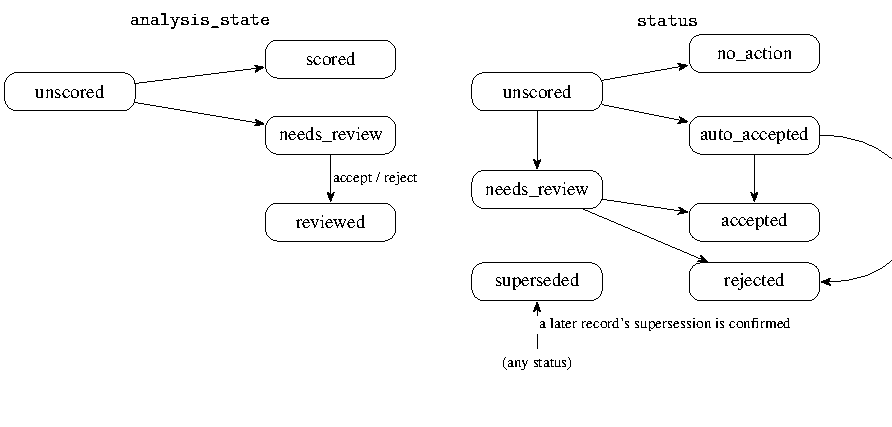
\includegraphics[width=\linewidth,height=0.70\textheight,keepaspectratio]{illustrations/fig_p64_68.pdf}
\caption{State diagrams for analysis\_state and status.}
\label{fig:state}
\end{figure}

\subsection{Build and release}

Figure~\ref{fig:cicd} shows how a change reaches users. The frontend is built by Vercel on every push. The backend is deployed to staging only from a main commit that passed all three CI jobs; a manual deploy or rollback needs an exact commit and a typed confirmation.

\begin{figure}[!htbp]
\centering
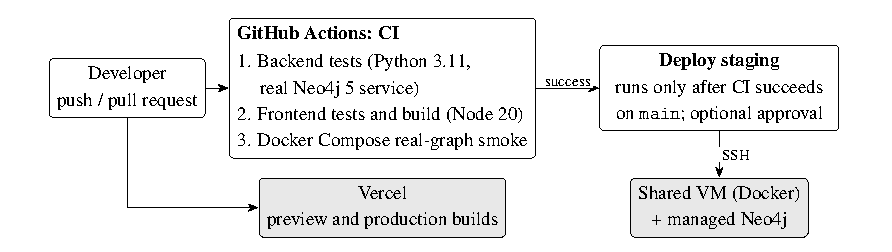
\includegraphics[width=\linewidth,height=0.70\textheight,keepaspectratio]{illustrations/fig_p64_405.pdf}
\caption{CI/CD pipeline.}
\label{fig:cicd}
\end{figure}
